\newpage
\phantomsection
%\addcontentsline{toc}{chapter}{Appendix: Pattern recognition}

%\begin{appendix}

\chapter[Isometric and non-isometric task identification]{Identification of isometric and non-isometric upper-limb tasks using HD-EMG}
\label{RIAI}
\textbf{Published as:} 
Rojas-Mart\'inez, M., Alonso, J.F., Jordani\'c, M., Romero, S., Ma\~nanas, M.A.
Identificación de tareas isométricas y dinámicas del miembro superior basada en EMG de alta densidad.
\textit{Revista Iberoamericana de Autom\'atica e Inform\'atica industrial (RIAI)}, Accepted for publication, 2017

doi: ------------------

Impact Factor: 0.500; Position: 57 of 60 (Q4) AUTOMATION AND CONTROL SYSTEMS; 25 OF 26 (Q4) ROBOTICS.


\textbf{Abstract:} Identification of tasks and estimation of volitional movement based on electromyography (EMG) constitute a known problem that involves different areas in the field of expert systems and particularly pattern recognition, with many possible applications in assistive and rehabilitation devices. The obtained information can be very useful to control exoskeletons or robots used in active rehabilitation processes. The emerging method of high-density electromyography (HD-EMG) opens up new possibilities to extract neural information, and it has already been reported that the spatial distribution of HD-EMG intensity maps is a valuable feature in the identification of isometric tasks.

This study explores the use of the spatial distribution of myoelectric activity and carries out a task identification during dynamic exercises at different velocities which are much closer to the ones commonly used during therapy. To this end, HD-EMG signals were recorded in a group of healthy subjects while performing a set of isometric and dynamic upper limb tasks. The results show that spatial distribution is a very useful feature in the identification not only of isometric contractions but also of dynamic contractions, so it can be very useful to improve the control of rehabilitation devices, making it more natural and permitting to adapt better to the user.

\textbf{Keywords:}  bioengineering; electromyography; neuromuscular; rehabilitation

\section{Introduction}
Every year there are about half million spinal cord injuries and 15 million strokes. These injuries can have an impact on the motor control, resulting in uncoordinated movements, lack of force, and spasticity. In these cases, robot-assisted therapies can be used to stimulate neuroplasticity \citep{vanPepen2004}. If the movement intention of a patient could be extracted in real time, this information could be used to optimally control assistive devices based on the patient's needs, maximizing the benefits of the therapy \citep{Hogan2006}.

The use of the spatial information of the myoelectric activation maps is a novel method that can achieve high results of task identification, both in healthy subjects \citep{Stango2015}, but also in patients with incomplete spinal cord injury \citep{Rojas-Martinez2013, Jordanic2016a, Jordanic2016b}. This study analyses the possibility of using the features extracted from these maps for the identification of a set of isometric contractions performed at subjective force levels, and also for the identification of dynamic contractions. Upper-limb motor tasks were recorded in a group of healthy subjects, consisting of hand displacements over a horizontal plane, involving mostly shoulder movements. These tasks were selected because they are similar to those usually involved in therapy with rehabilitation robots \citep{Badesa2014}.


\section{Methodology}

\subsection{Experimental protocol}
Five male subjects participated in the study (age: 24.8 $\pm$ 6.1 years, height: 178.6 $\pm$ 10.2 cm, weight: 76.8 $\pm$ 13.8 kg). They had no neuromuscular or musculoskeletal disorders of the upper limb prior to the recording. HD-EMG signals of muscles associated to the shoulder movement, namely \textit{biceps brachii}, \textit{triceps brachii}, \textit{pectoralis major}, and upper part of the \textit{trapezius}, were recorded on the dominant side using two EMG amplifiers (EMG-USB, OT-Bioelettronica, Tur\'in, Italy) with synchronized sampling (2048 Hz sampling frequency). Using four 2D electrode arrays manufactured in our laboratory, 228 differential EMG channels were measured. Electrode arrays were designed as silver-plated eyelets embedded in the hydrophobic fabric with inter-electrode distance of 10 mm. Arrays were placed so that the center of the array would be positioned following the guidelines of the SENIAM project \citep{Hermens1999}.

Experimental protocol was divided in two parts: a) recording of isometric contractions, and b) recording of dynamic contractions.
During the recording of the isometric contractions, subjects were seated upright with their back straight, elbow flexed at approximately 90 degrees, and shoulder in the neutral position (see figure \ref{fig:4-1}A). Maintaining this position, subjects performed three tasks, pushing a fixed object positioned directly in front of them forward, leftward, and rightward. Each of these tasks was realized at three different effort levels: low, medium, and high. Effort levels were chosen by the subjects following their own perception of the exerted force. In addition, HD-EMG was also recorded during the rest state. Each contraction had the duration of ten seconds with two minute rest period between contractions.

For the recording of dynamic contractions, subjects were asked to maintain the previously described posture (straight back and elbow flexed at 90 degrees) and to displace an object over the horizontal plane, following the predefined trajectory depicted in figure \ref{fig:4-1} as follows:

\begin{enumerate}[a)]
\item From the center of the plane, located at approximately 30 cm in front of the subject, until full extension of the shoulder, and return to the center.
\item From the center to a point located approximately 40 cm leftward, following the trajectory perpendicular to the previous one, and return to the center.
\item Repeat the same movement in the other direction, until the point located approximately 40 cm rightward, and return to the center.
\end{enumerate}

Each movement sequence was performed two times at two different velocities, fast and slow, based on the subject's perception, but without change of speed during the sequence. In addition to HD-EMG, positioning signal was also recorded. Proximity sensors were used that generated a signal each time the subject would reach one of the end-points of the trajectory (see figure \ref{fig:4-1}B).

\begin{figure*}[t!]
    \centering
    \begin{subfigure}[t]{0.45\textwidth}
        \centering
        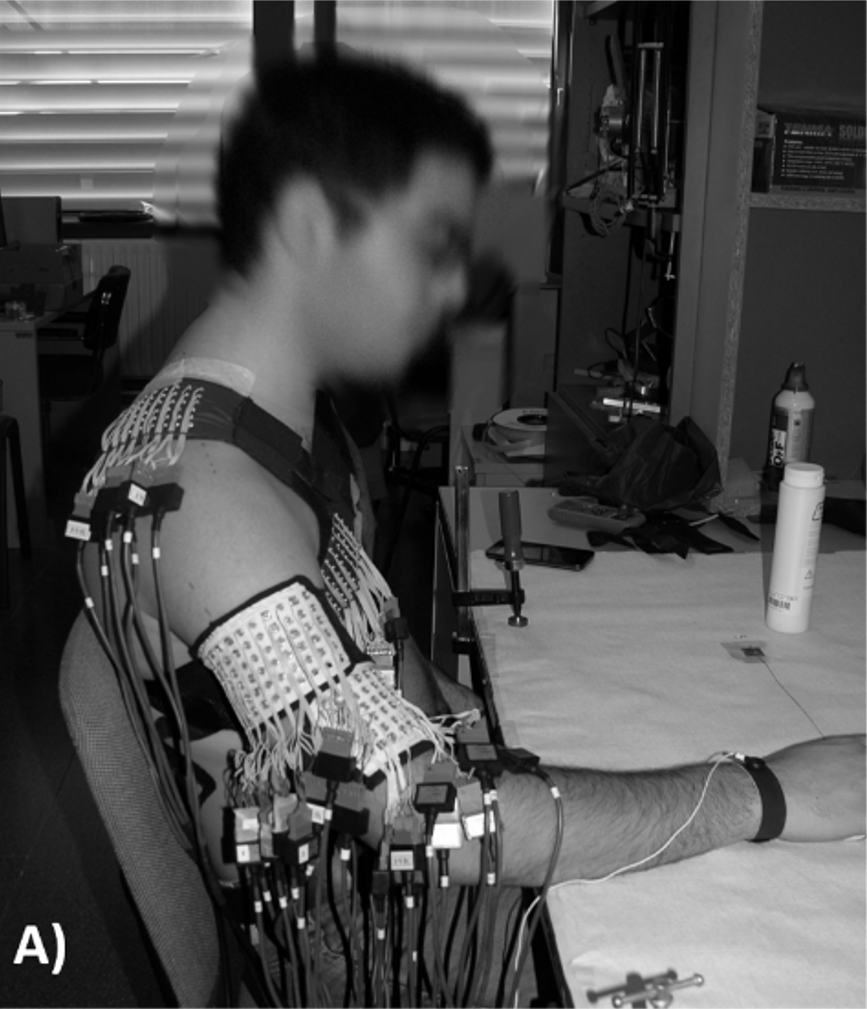
\includegraphics[height=2.9in]{Images/figure4_1a.png}
   
    \end{subfigure}%
    ~ 
    \begin{subfigure}[t]{0.45\textwidth}
        \centering
        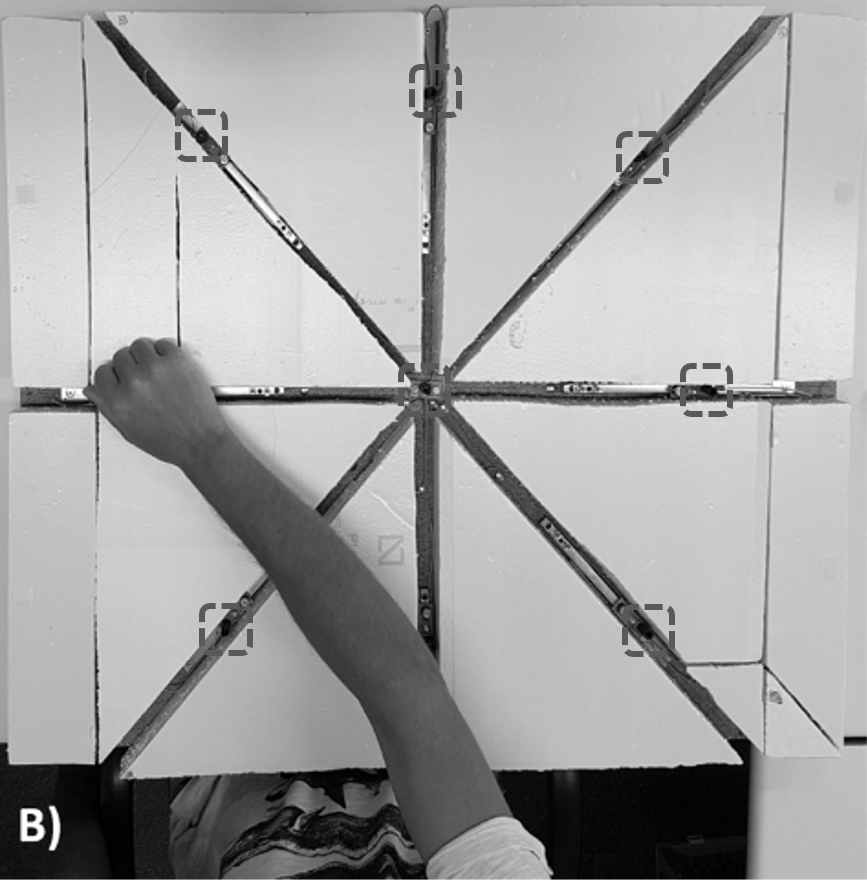
\includegraphics[height=2.9in]{Images/figure4_1b.png}
        
    \end{subfigure}
    \caption{Figure shows \textbf{A)} measurement equipment and the position of the subject during the experimental protocol, and \textbf{B)} experimental plane in which the tasks were performed. Position sensors are marked by dashed rectangles.}
\label{fig:4-1}
\end{figure*}


\subsection{Signal processing}
The recorded signals were filtered using a 4\textsuperscript{th} order Butterworth filter with zero-phase. Additionally, signals were filtered using an adaptive filter for reducing the power line interference.

Afterwards, signals were divided in 250 ms time windows without overlapping, and the RMS value was calculated for each channel. Using these values, activation map $HM$ was calculated for each time window as:
\begin{equation} \label{eq:4-1}
HM_{i,j} = \sqrt{\frac{\sum_n{sEMG_{i,j}^2 (n)}}{N}}
\end{equation}

, where $N=512$ samples (corresponding to time window of 250 ms), $i$ and $j$ are positions (row and column in the electrode array) of the sEMG channel, which correspond to the position ($i,j$) of the pixel in the activation map $HM$. The channels identified as artifacts were substituted using the triangle-based cubic interpolation \citep{Rojas-Martinez2012}.

From these activation maps the following features were extracted: logarithm of the average intensity of the map (Ilog), and the center of gravity (CG). In the first case, it was already shown that the logarithmic transform is useful in the identification of effort levels \citep{Rojas-Martinez2012}, and in the second case, it was shown that the spatial distribution of myoelectric activity changes with the force level \citep{Holtermann2005}, and with the isometric task intention \citep{Jordanic2016a}.

On the other hand, a position signal recorded during dynamic part of the protocol was used to partition the HD-EMG signal into segments corresponding to each of the movements described in the protocol.


\subsection{Movement classification}
The classification was realized for each subject individually, both for the isometric tasks, and for the dynamic tasks. For the isometric tasks, two types of classification were considered:

\begin{enumerate}[a)]
\item identification of four tasks regardless of the effort level (rest, push forward, push leftward, push rightward)

\item identification of tasks and effort levels (identification of three tasks at three different effort levels, and the rest state)
\end{enumerate}

The identification of the isometric tasks was performed to validate the experimental protocol. Although in our previous work we managed to identify isometric tasks with high sensitivity and precision, using both intensity and spatial features, the tasks considered in that studies were related to the elbow, and not to the shoulder \citep{Jordanic2016a, Jordanic2016b, Rojas-Martinez2013}.

For the dynamic task, the identification consisted of the classification of each of the following tasks:
 
\begin{enumerate}[a)]
\item move forward
\item return back to the center
\item move leftward
\item return back to the center
\item move rightward
\item return back to the center
\end{enumerate}

For the task identification, a classifier based on the linear discriminant analysis (LDA) was used, a technique often used in myoelectric pattern recognition because of its properties relating speed and low computational complexity \citep{Zhou2007}.

In the case of isometric contractions, database was separated in two groups, training set, consisting of 60\% of the available data, and test set, consisting of 40\% of the available data. This data separation, followed by the training and classification was repeated 100 times in order to minimize possible statistical errors (i.e. the hold-out validation method). The identification results reported in the study were obtained after averaging over all iterations.

In the case of dynamic contractions, the classifier was trained using the observations recorded in one recording sequence (both for slow and fast movements), and validated using the observations recorded in the other sequence. Afterwards, the training set and the test set were swapped and the identification was repeated. The reported results are the average of these two identifications. As in the previous case, this type of validation was used to reduce possible statistical error, although it is possible that in the second recording the subject learned how to control the velocity and perform the exercise better.

Finally, the performance of the classification was expressed in terms of sensitivity (S) and precision (P) \citep{Farina2001}, calculated as:
\begin{equation}
S = \frac{TP}{TP+FN}
\end{equation}
\begin{equation}
P = \frac{TP}{TP+FP}
\end{equation}
, where TP is the number of true positives, that is, correctly classified samples, FP is the number of false positives, which indicate the number of wrongly classified samples to a certain class, and FN is the number of false negatives, that is, the number of samples incorrectly classified to another class. The sensitivity (S) and precision (P) were obtained for each of the classes, and the averaged results were calculated.


\section{Results}
\subsection{Activation maps}
In figure \ref{fig:4-2} an example of activation maps of \textit{pectoralis major} are shown. Different activation patterns can be observed during the performance of dynamic tasks. It should be noted that the activation intensity depends on the task, presenting the highest activation (in mV) during the return from full forward extension to the center of the plane, and the reverse. Also, it can be noted that the spatial distribution changes depending on the exercise, for example, during the contraction associated with the forward movement (see figure \ref{fig:4-2}a), the activation is located at the left side of the map (columns 1 to 3), whereas in the rightward movement (see figure \ref{fig:4-2}b), the area with higher activity is located in the right part of the map (column 8, rows 2 to 4). Although only maps of \textit{pectoralis major} are shown, similar differences can be found in the remaining three muscles, which is used as a feature in the identification. 

\begin{figure}[ht]
\centering
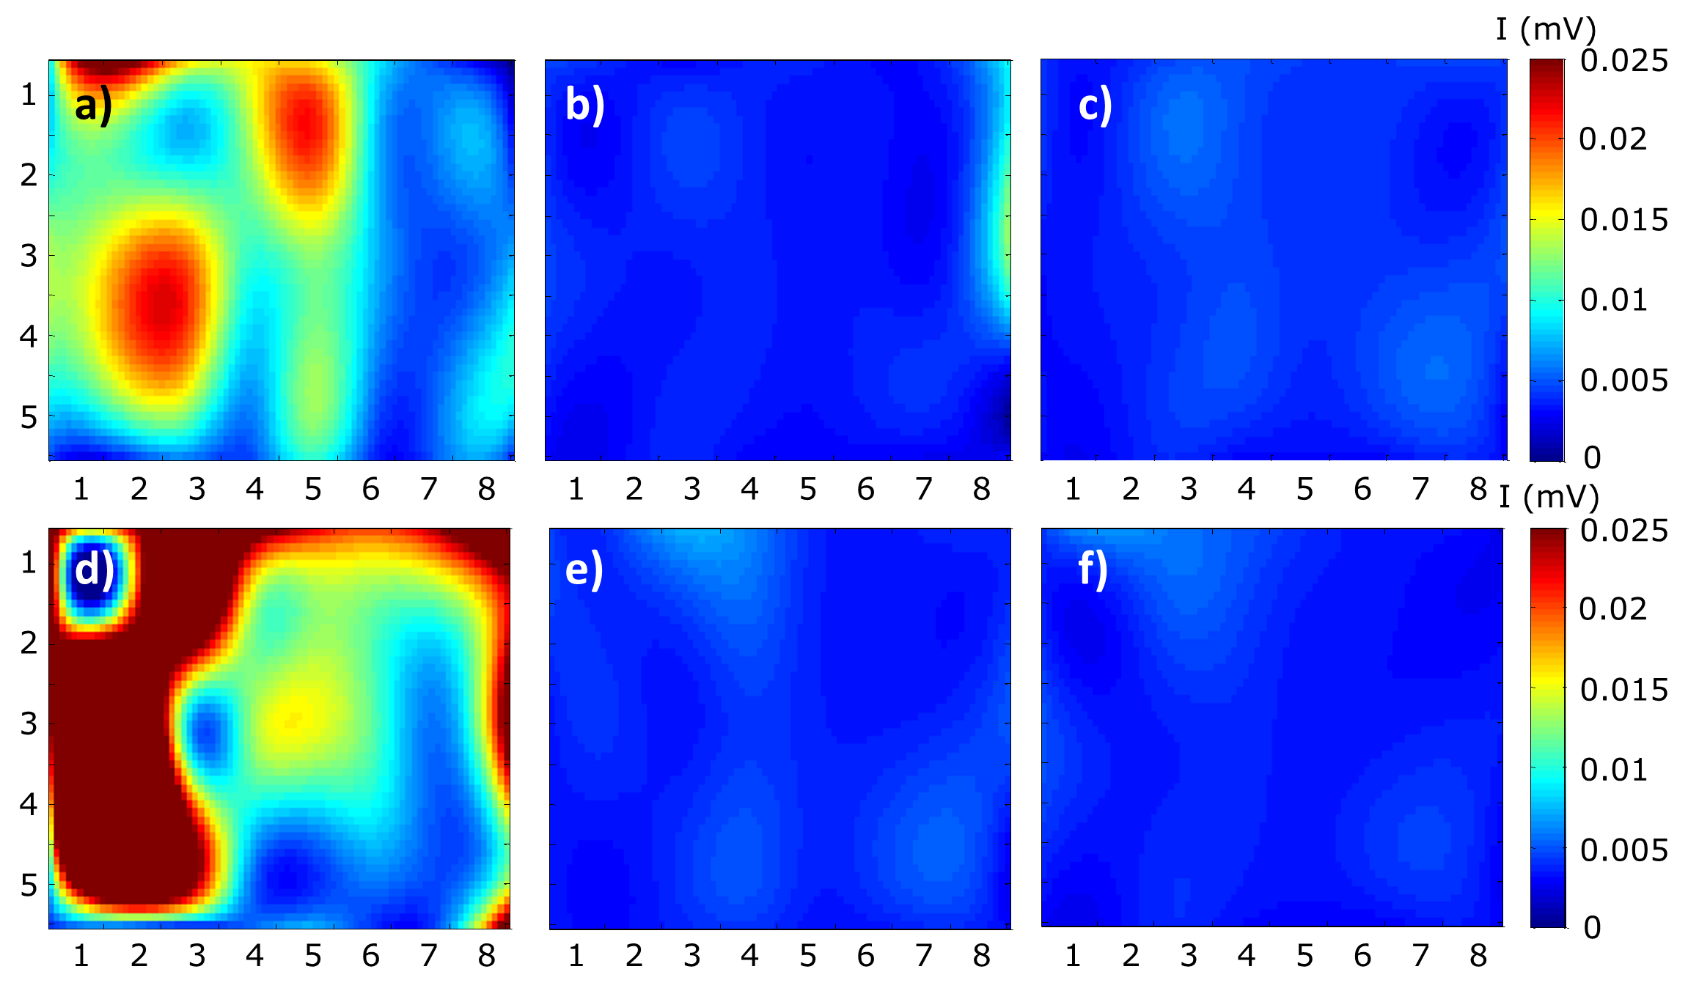
\includegraphics[width=0.99\textwidth]{Images/figure4_2.png}
\caption{Activation maps of \textit{pectoralis major} of one of the subjects. Up. Movement from the central point a) forward, b) rightward, and c) leftward. Down. Movement toward the center from  d) ahead, e) right, and f) left.}
\label{fig:4-2}
\end{figure}

\subsection{Isometric task identification}
To test if the spatial distribution of intensity improves the identification, two types of identification were performed: the identification based only on intensity features, and the identification based on the combination of intensity and spatial features. Additionally, identification of task was performed (forward, rightward, leftward, and rest), and the identification of task and effort levels. The results of the task identification, regardless of the effort level are shown in table \ref{tb:4-1}, whereas the results of the identification of task and effort level are shown in table \ref{tb:4-2}.

\begin{table}[h!]
\centering
\caption{Results of the identification of isometric tasks using the Ilog features and the combination of Ilog and CG features. The results are presented as the mean and the standard deviation calculated across five subjects.}
\label{tb:4-1}
\begin{tabular}{lccccc}
 
              & \multicolumn{2}{c}{\textbf{Ilog}}                            & \multicolumn{2}{c}{\textbf{Ilog + CG}}                       \\
\textbf{Task} & \textbf{Sensitivity}     & \textbf{Precision}       & \textbf{Sensitivity}     & \textbf{Precision}       \\ \hline
                         &                                           &          &          &                   \\
Forward       & 73 $\pm$ 13              & 77.1 $\pm$ 15            & 92.1 $\pm$ 6.9           & 93.6 $\pm$ 6.4           \\
Rightward     & 83.5 $\pm$ 16            & 92 $\pm$ 9.4             & 96.2 $\pm$ 4.9           & 95.9 $\pm$ 3.9           \\
Leftward      & 85.8 $\pm$ 14            & 87.3 $\pm$ 13            & 96.1 $\pm$ 5.4           & 97.8 $\pm$ 5             \\
Rest          & 98.7 $\pm$ 2.1           & 87.1 $\pm$ 3.2           & 100 $\pm$ 0              & 98.5 $\pm$ 3.4           \\ 
\textbf{Mean} & \textbf{85.3 $\pm$ 11.2} & \textbf{85.9 $\pm$ 10.2} & \textbf{96.1 $\pm$  4.3} & \textbf{96.4  $\pm$ 4.7}
\end{tabular}
\end{table}

\begin{table}[h!]
\centering
\caption{Results of the identification of isometric tasks and effort levels using the Ilog features and the combination of Ilog and CG features. The results are presented as the mean and the standard deviation calculated across five subjects.}
\label{tb:4-2}
\begin{tabular}{llcccc}
              & \multicolumn{2}{c}{\textbf{Ilog}}                            & \multicolumn{2}{c}{\textbf{Ilog + CG}}                       \\
\textbf{Task} & \textbf{Force} & \textbf{Sensitivity}                          & \textbf{Precision}                           & \textbf{Sensitivity}                         & \textbf{Precision}                          \\ \hline
              &                &                                               &                                              &                                             &                                             \\
              & low            & 91.4 $\pm$ 14                                 & 89.8 $\pm$ 12                                & 99 $\pm$ 2.3                                & 99.2 $\pm$ 1.7                              \\
Forward       & medium         & 86.4 $\pm$ 25                                 & 88.8 $\pm$ 16                                & 96.7 $\pm$ 7.5                              & 99.4 $\pm$ 1.4                              \\
              & high           & 87.7 $\pm$ 14                                 & 89.9 $\pm$ 14                                & 95.8 $\pm$ 6                                & 98.5 $\pm$ 3.4                              \\ \hline
              & low            & 98.3 $\pm$ 3.7                                & 89.4 $\pm$ 11                                & 97.7 $\pm$ 3.6                              & 94.6 $\pm$ 7.5                              \\
Rightward     & medium         & 90.4 $\pm$ 18                                 & 91.3 $\pm$ 6.5                               & 98.3 $\pm$ 3.7                              & 98.3 $\pm$ 3.9                              \\
              & high           & 98.3 $\pm$ 3.9                                & 100 $\pm$ 0                                  & 100 $\pm$ 0                                 & 99.2 $\pm$ 1.7                              \\ \hline
              & low            & 96 $\pm$ 5.1                                  & 92.1 $\pm$ 8.3                               & 96.9 $\pm$ 7                                & 95.2 $\pm$ 7.3                              \\
Leftward      & medium         & 85.7 $\pm$ 5.9                                & 85.3 $\pm$ 11                                & 94.4 $\pm$ 7.8                              & 94.8 $\pm$ 7.4                              \\
              & high           & 93.9 $\pm$ 7.1                                & 96 $\pm$ 7.2                                 & 98.3 $\pm$ 3.7                              & 97 $\pm$ 6.6                                \\ \hline
Rest          &                & \multicolumn{1}{l}{97.5 $\pm$ 5.6}            & \multicolumn{1}{l}{98.5 $\pm$ 3.4}           & \multicolumn{1}{l}{100 $\pm$ 0}             & \multicolumn{1}{l}{99 $\pm$ 2.2}            \\
\textbf{Mean} & \textbf{}      & \multicolumn{1}{l}{\textbf{92.6  $\pm$ 10.2}} & \multicolumn{1}{l}{\textbf{92.1  $\pm$ 8.9}} & \multicolumn{1}{l}{\textbf{97.7 $\pm$ 4.2}} & \multicolumn{1}{l}{\textbf{97.5 $\pm$ 4.3}}
\end{tabular}
\end{table}

It can be seen that by adding the center of gravity to intensity features, results improve approximately 10\% in the case of the task identification and 5\% in the case of the identification of task and effort level. Moreover, since when using center of gravity, standard deviation is smaller, it can be concluded that spatial distribution has a positive effect on the identification.


\subsection{Dynamic task identification}
In the case of dynamic task identification, 6 classes were considered: move forward and return, move leftward and return, and move rightward and return.

Tables \ref{tb:4-3} and \ref{tb:4-4} show the results obtained by averaging the results for each patient, using only intensity features (table \ref{tb:4-3}), and combination of intensity and spatial features (table \ref{tb:4-4}). As in isometric contractions, identification results are higher when combining intensity and spatial features.

\begin{table}[h!]
\centering
\caption{Identification of six dynamic contractions based on the intensity features, separately for slow movements and fast movements. The results are presented as the mean and the standard deviation calculated across five subjects.}
\label{tb:4-3}
\begin{tabular}{llcccc}
                   &           & \multicolumn{2}{c}{\textbf{Slow}}          & \multicolumn{2}{c}{\textbf{Fast}}           \\
                   &           & \textbf{Sensitivity} & \textbf{Precision}  & \textbf{Sensitivity} & \textbf{Precision}   \\ \hline
                   &           &                      &                     &                      &                      \\
From the center    & Leftward  & 60.7 $\pm$ 12.6          & 68.8 $\pm$ 7.9          & 77.2 $\pm$ 14.1          & 74.9 $\pm$ 13.5          \\
                   & Rightward & 87.7 $\pm$ 7.8           & 79.6 $\pm$ 8.7          & 77.2 $\pm$ 14.3          & 75.7 $\pm$ 12.0          \\
                   & Forward   & 77.9 $\pm$ 9.9           & 74.8 $\pm$ 10.1         & 76.8 $\pm$ 13.6          & 77.0 $\pm$ 10.6          \\ \hline
Toward center from & Ahead     & 73.4 $\pm$ 11.8          & 74.7 $\pm$ 11.1         & 80.4 $\pm$ 14.2          & 75.5 $\pm$ 9.5           \\
                   & Right     & 68.8 $\pm$ 11.5          & 75.7 $\pm$ 12.1         & 85.4 $\pm$ 9.3           & 78.8 $\pm$ 10.4          \\
                   & Forward   & 71.8 $\pm$ 9.0           & 72.9 $\pm$ 8.3          & 78.3 $\pm$ 20.9          & 71.9 $\pm$ 15.6          \\ \hline
\textbf{Mean}      & \textbf{} & \textbf{73.4 $\pm$ 10.4} & \textbf{74.4 $\pm$ 9.7} & \textbf{79.2 $\pm$ 14.4} & \textbf{75.7 $\pm$ 11.9}
\end{tabular}
\end{table}


\begin{table}[h!]
\centering
\caption{Identification of six dynamic contractions based on the combination of intensity and spatial features, separately for slow movements and fast movements. The results are presented as the mean and the standard deviation calculated across five subjects.}
\label{tb:4-4}
\begin{tabular}{llcccc}
                   &           & \multicolumn{2}{c}{\textbf{Slow}}           & \multicolumn{2}{c}{\textbf{Fast}}           \\
                   &           & \textbf{Sensitivity} & \textbf{Precision}   & \textbf{Sensitivity} & \textbf{Precision}   \\ \hline
                   &           & \multicolumn{1}{l}{} & \multicolumn{1}{l}{} & \multicolumn{1}{l}{} & \multicolumn{1}{l}{} \\
From the center    & Leftward  & 85.0 $\pm$ 13.1          & 83.1 $\pm$ 5.7           & 94.4 $\pm$ 11.4          & 94.0 $\pm$ 13.3          \\
                   & Rightward & 94.8 $\pm$ 3.4           & 91.9 $\pm$ 7.9           & 95.6 $\pm$ 9.2           & 90.6 $\pm$ 14.6          \\
                   & Forward   & 84.4 $\pm$ 11.0          & 86.7 $\pm$ 11.0          & 95.4 $\pm$ 9.2           & 90.4 $\pm$ 13.8          \\ \hline
Toward center from & Ahead     & 92.3 $\pm$ 7.1           & 92.4 $\pm$ 12.8          & 93.7 $\pm$ 14.1          & 93.7 $\pm$ 14.1          \\
                   & Right     & 85.1 $\pm$ 6.2           & 86.7 $\pm$ 6.6           & 96.6 $\pm$ 7.1           & 92.1 $\pm$ 12.1          \\
                   & Forward   & 81.0 $\pm$ 5.6           & 89.7 $\pm$ 7.4           & 91.8 $\pm$ 11.0          & 85.5 $\pm$ 14.0          \\ \hline
\textbf{Mean}      & \textbf{} & \textbf{87.1 $\pm$ 7.7}  & \textbf{88.4 $\pm$ 8.6}  & \textbf{94.6 $\pm$ 10.3} & \textbf{91.0 $\pm$ 13.6}
\end{tabular}
\end{table}

Higher variability can be observed compared to the isometric task identification, as well as lower sensitivity and precision, as could be expected since the dynamic contractions represent a more complex problem. Finally, it should be noted that although the mean identification results of fast movements are higher than slow movements, the variability is higher in the identification of fast movements. Therefore, it cannot be said with certainty that fast movements can be identified with higher identification results.


\section{Conclusions}

Results show that in all cases identification can be improved by adding spatial features, i.e., center of gravity to the intensity features. This fact implies that task-dependent patterns exist in the spatial domain, both for isometric tasks and for dynamic tasks. Besides, adding features based on the spatial distribution improved average identification results and reduced its variability therefore improving the robustness of the identification.

This results confirm previous findings in the literature \citep{Hargrove2007, Farina2008, Jordanic2016a, Zhou2007} that there is a  neuromuscular compartmentalization within the muscles, and that different muscle areas activate during different tasks. %Por lo tanto, es posible que estos hallazgos puedan extenderse al músculo Pectoralis Major que no había sido evaluado previamente en nuestros estudios anteriores.

Moreover, in the case of isometric contractions, besides identifying only task (forward, rightward, and leftward), it is also possible to identify force level, which enables simultaneously controlling task and force, which is an important step towards the control of external devices in a natural way. 

On the other hand, identification results of dynamic contractions are lower than the identification results of the isometric contractions. These results can be expected since dynamic contractions imply joint movement and shortening of the muscle fibers, which has an effect over the sEMG signal and increases the complexity of the classification problem. Moreover, the velocity of the movement was decided by the subject, which makes it subjective, and more difficult to classify, as would be the case in a real rehabilitation scenario. In spite of these difficulties, the obtained results are very promising (sensitivity and precision close to 90\%), but should be improved further in terms of identification indices and robustness.

The overall results of the identification of fast and slow movements are similar. Although the identification of fast movements has higher identification indices, the standard deviation is also higher ($>$10\%), and, therefore, it cannot be concluded with certainty that the  identification depends on the speed of the movement. To establish this relationship, more tests should be performed on a bigger database.

As a general conclusion, it was demonstrated that the proposed methodology and the obtained results are promising and that the information extracted from the HD-EMG can be useful for controlling of external devices, e.g. rehabilitation robots.

Future works should consider the extension of the protocol to patients with neuromuscular impairments, where the motion intention could be extracted from intensity and spatial domain of HD-EMG recordings in order to control external devices like rehabilitation robots. 

\section{Acknowledgments}
The authors are grateful to Ignasi Gallardo for his collaboration in the development of the study.
This work has been partially supported by the project ROBERT of the CIBER-BBN, and by the Spanish Ministry of Economy and Competitiveness (project DPI2014-59049-R).

%\end{appendix}